È possibile fare ricerche di progetti utilizzando come filtro l'username di un utente oppure il nome di un progetto.
\newline
Per eseguire una ricerca è sufficiente recarsi sulla pagina iniziale tramite l'utilizzo del pulsante \textbf{PREMI} posto nell'angolo superiore sinistro dello schermo, scrivere la chiave di ricerca nell'apposita casella di testo, selezionare il filtro che si vuole utilizzare (Users o Project) e infine premere il tasto \textbf{Search}.

\begin{figure}[h] 
	\centering 
	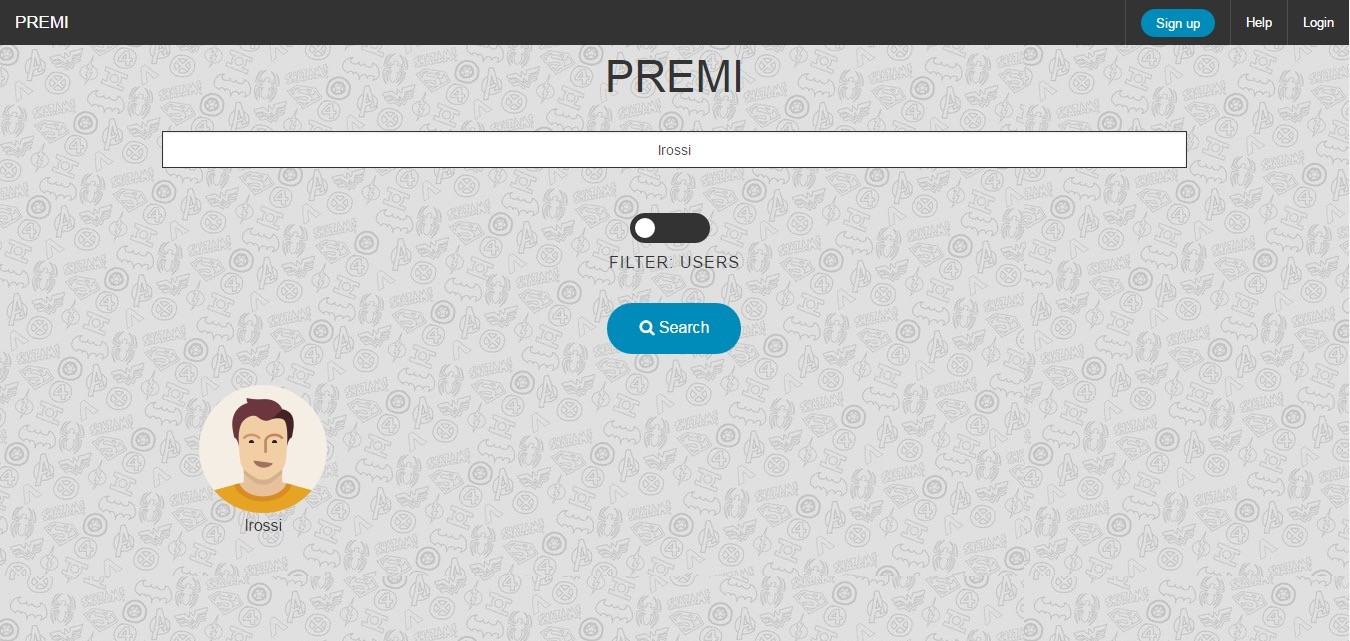
\includegraphics[scale=0.40] {img/ricerca}
	\caption{Ricerca} 
\end{figure}


\noindent I risultati della ricerca verranno mostrati sotto il pulsante \textbf{Search}, come mostrato nella figura sottostante.

\begin{figure}[h] 
	\centering 
	
\includegraphics[scale=0.40] {img/ricercaris}
	\caption{Risultati ricerca} 
\end{figure}

\noindent Nel caso in cui la ricerca non abbia trovato alcun risultato, verrà segnalato con la dicitura \textbf{No results} come è possibile notare nella figura.

\begin{figure}[H] 
	\centering 
	
\includegraphics[scale=0.40] {img/noresults}
	\caption{Nessun risultato di ricerca} 
\end{figure}